\chapter{探测器、时钟和事件表}
\label{chap:06}

\begin{chapteropening}
第五章把强度干涉写成一个很小的相关峰，典型幅度可以只有 \(10^{-6}\)。这样的信号不会自动出现在论文图上。它先要经过镜面、滤光片、探测器、放大器、数字化器、时钟、数据格式和质量筛选。每一步都会改变事件率、时间戳、响应宽度或背景比例，因此也会改变最终的 \(g^{(2)}\)、\(|V|^2\) 或脉冲到达时刻。

本章的问题是：一台真实望远镜怎样把光子变成可复现的事件表？事件表不是普通光变曲线。它保留每个候选光子的时间、通道、波长、偏振和质量信息，使同一份数据以后还能重新分箱、重新选频、重新做延迟校正，或投影成光变曲线、功率谱、相关函数和脉冲相位。AquEYE/Iqueye、VERITAS-SII、MAGIC-SII、MKID 仪器和现代 TCSPC/White Rabbit 系统都说明了同一件事：相关函数里的时间尺度、效率因子和噪声项，最终来自探测器、电子学和时钟系统 \citep{2009JMOp...56..261B,2009A&A...508..531N,2015SPIE.9504E..0CZ,2020NatAs...4.1164A,2024MNRAS.529.4387A,2013PASP..125.1348M,2018PASP..130f5001M,2020RScI...91a3108W}。
\end{chapteropening}

\section{事件表为什么要保留原始信息}

第 \ref{chap:01} 章式 \eqref{eq:event-row} 给出了全书使用的最小事件行；第 \ref{chap:02} 章说明，把事件过早平均成图像、光谱或光变曲线，会丢掉许多联合概率。在仪器层，图像和事件表的区别很具体。图像把一段曝光内的光子数累加到像素上；事件表则保留每个触发事件的时间、探测器通道、望远镜编号、波长或滤光片、偏振通道、权重和质量标记。对普通测光，二者常常足够接近；对纳秒到皮秒计时、二阶相关、脉冲星折叠或快速遮掩，早期累加会直接删除待测信号。

Iqueye 的设计就是一个好例子。它把所有光子以时间标签保存下来，然后离线选择从 24.41 ps 到分钟级的任意时间 bin。对 \(\zeta\) Ori 的观测产生约 \(2\times10^{10}\) 个光子事件，数据量约 78 GB \citep{2009A&A...508..531N,2019CoSka..49...85Z}。这说明事件表不是小型辅助文件，而是真实望远镜会面对的主要数据产品。

原始事件可以写成
\begin{equation}
  \mathcal{E}^{\rm raw}_q =
  \left(n_q,\ a_q,\ d_q,\ c_q,\ p_q,\ f_q,\ w_q\right),
  \qquad
  t^{\rm raw}_q=t_0+n_q\,\delta t+\epsilon_{\rm roll}.
  \label{eq:ch06-raw-event}
\end{equation}
\begin{formulaexplain}
\(\mathcal E_q^{\rm raw}\) 是第 \(q\) 个原始事件；\(n_q\) 是时钟 tick，\(\delta t\) 是 tick 时长，\(t_0\) 是段起点，\(\epsilon_{\rm roll}\) 处理计数器溢出。它把电子记录变成最早的事件时间。
\end{formulaexplain}
下标 \(q\) 标记第 \(q\) 个事件。\(n_q\) 是电子计数器的整数时钟 tick；\(\delta t\) 是一个 tick 对应的时间，单位是秒；\(t_0\) 是记录段的起始时间；\(\epsilon_{\rm roll}\) 处理计数器溢出、分段或 rollover。现代时间数字转换器可在 \(10^{-11}\)--\(10^{-10}\,{\rm s}\) 量级取样，商用多通道 TCSPC 系统的基本时间分辨率可为 80 ps，Iqueye 的 TDC 量化步长为 24.41 ps \citep{2009A&A...508..531N,2020RScI...91a3108W}。\(a_q\) 是望远镜或站点编号，\(d_q\) 是探测器编号，\(c_q\) 是波长通道或滤光片编号，\(p_q\) 是偏振通道，\(f_q\) 是质量标记，\(w_q\) 是事件权重。溢出、丢包、饱和、云、指向异常和电子学异常都应进入 \(f_q\)，否则后续相关函数中的异常峰很难被追溯。

\begin{figure}[tbp]
\centering
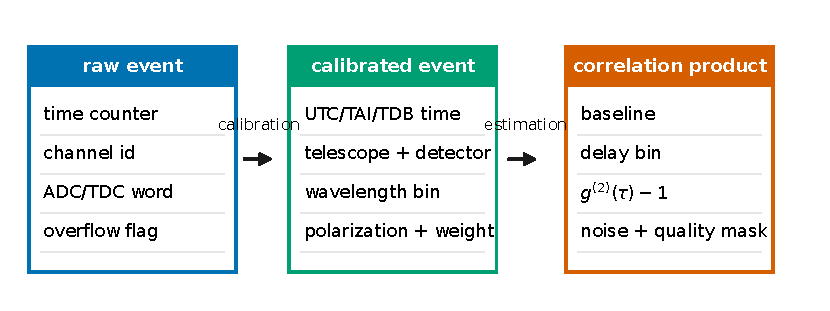
\includegraphics[width=0.96\linewidth]{figures/generated/chapter_06/ch06_event_table_schema.pdf}
\caption{事件数据从原始电子记录流向标定事件表，再流向相关函数产品。原始层保存计数器时间、通道编号和溢出标记；标定层把时间转换到统一时间尺度，并加入望远镜、波长、偏振和权重；相关产品层才记录基线、延迟 bin、相关幅度和噪声估计。若在第一层就只保存光变曲线，后面的时钟、波长和偏振选择都无法重新执行。}
\label{fig:ch06-event-table-schema}
\end{figure}

标定事件表把原始计数器时间变成可比较的物理时间：
\begin{equation}
  t^{\rm cal}_q =
  t^{\rm raw}_q
  +\Delta_{\rm clk}(t_q)
  +\Delta_{\rm elec}(a_q,d_q)
  +\Delta_{\rm det}(\lambda_q,d_q)
  -\frac{\mathbf{r}_{a_q}(t_q)\cdot\hat{\mathbf{s}}}{c}.
  \label{eq:ch06-calibrated-time}
\end{equation}
\begin{formulaexplain}
\(t_q^{\rm cal}\) 是校正后的事件时间；\(\Delta_{\rm clk}\)、\(\Delta_{\rm elec}\)、\(\Delta_{\rm det}\) 分别改正时钟、电子链路和探测器延迟；最后一项扣除几何光行时。它把不同站点放到共同时间轴。
\end{formulaexplain}
\(\Delta_{\rm clk}\) 是站点时钟相对统一时间尺度的偏移，单位秒；短时间内可以是几十皮秒到纳秒，跨夜合并时还要处理 GPS、TAI、UTC、TT 或 TDB 的转换。\(\Delta_{\rm elec}\) 是电缆、放大器、鉴别器、ADC/TDC 通道产生的固定或缓慢漂移延迟，常用脉冲源和环回链路标定。\(\Delta_{\rm det}\) 是探测器内部延迟，可能依赖波长、偏置电压、温度和脉冲高度；SNSPD 的探测延迟甚至会随光子能量变化 \citep{2020NaPho..14..250K,2020Optic...7.1649R}。最后一项是几何延迟，\(\mathbf{r}_{a_q}\) 是站点相对参考点的位置向量，\(\hat{\mathbf{s}}\) 是源方向单位向量，\(c\) 是光速。100 m 基线给出最高约 333 ns 的几何延迟，1 km 基线给出约 \(3.3\,\mu{\rm s}\)，远大于皮秒级探测器抖动。

数据率由事件率和每个事件占用的字节数决定：
\begin{equation}
  \dot{M}
  \simeq
  N_{\rm tel}\,N_{\rm ch}\,R_{\rm evt}\,N_{\rm byte}.
  \label{eq:ch06-data-rate}
\end{equation}
\begin{formulaexplain}
\(\dot M\) 是数据率；\(N_{\rm tel}\) 是望远镜数，\(N_{\rm ch}\) 是通道数，\(R_{\rm evt}\) 是单通道事件率，\(N_{\rm byte}\) 是每事件字节数。它估算事件表或波形流的存储压力。
\end{formulaexplain}
\(\dot M\) 的单位是 byte s\(^{-1}\)。\(N_{\rm tel}\) 是望远镜数，\(N_{\rm ch}\) 是每台望远镜的独立通道数，\(R_{\rm evt}\) 是单通道事件率，\(N_{\rm byte}\) 是每个事件的存储大小。如果 \(N_{\rm tel}=4\)、\(N_{\rm ch}=8\)、\(R_{\rm evt}=10^6\,{\rm s^{-1}}\)、\(N_{\rm byte}=16\) byte，则 \(\dot M\simeq512\,{\rm MB\,s^{-1}}\)。连续波形采样会更高：VERITAS-SII 以 250 MS/s 连续数字化每台望远镜的 PMT 信号，单望远镜数据流约 250 MB/s，整次实验的数据量达到几十 TB \citep{2020NatAs...4.1164A}。事件表、波形流和实时相关器可以共存，区别在于压缩、筛选和相关计算发生在数据链的哪个阶段。

\Needspace{16\baselineskip}
\section{探测器怎样塑造事件率和间隔}

探测器的第一项作用是决定有多少入射光子变成电子事件。一个通道的平均探测率可写成
\begin{equation}
  R_{\rm det}
  =
  A_{\rm eff}
  \int_{\lambda_1}^{\lambda_2}
  F_\lambda(\lambda)\,
  T_{\rm opt}(\lambda)\,
  \eta_{\rm det}(\lambda)\,
  d\lambda
  +R_{\rm sky}+R_{\rm dark}.
  \label{eq:ch06-detected-rate}
\end{equation}
\begin{formulaexplain}
\(R_{\rm det}\) 是探测计数率；\(A_{\rm eff}\) 是有效面积；\(F_\lambda\)、\(T_{\rm opt}\)、\(\eta_{\rm det}\) 描述源光子、光路透过率和探测效率；\(R_{\rm sky},R_{\rm dark}\) 是背景。它给出事件率预算。
\end{formulaexplain}
\(A_{\rm eff}\) 是有效集光面积，单位 m\(^2\)；\(F_\lambda\) 是源的光子谱通量密度，单位 photons s\(^{-1}\) m\(^{-2}\) nm\(^{-1}\)；\(T_{\rm opt}\) 是镜面、滤光片、光纤、准直器和窗口的总透过率；\(\eta_{\rm det}\) 是探测器量子效率；\(R_{\rm sky}\) 是天空背景和杂散光计数率；\(R_{\rm dark}\) 是暗计数率。强度干涉的信噪比由源光子率和背景稀释后的强度起伏共同决定。MAGIC-SII 直接用 PMT 直流电流估计光子通量，并用背景像素修正夜天光贡献；VERITAS-SII 用 off-source 测量估计背景，再把相关幅度按恒星光占比修正 \citep{2020NatAs...4.1164A,2024MNRAS.529.4387A}。

不同探测器适合不同任务。PMT 的优势是面积大、增益高、ns 级脉冲和 Cherenkov 望远镜高速电子链路兼容；蓝光量子效率常在 \(20\%\)--\(40\%\)，VERITAS-SII 在 416 nm 使用的 PMT 量子效率约 \(30\%\) \citep{2020NatAs...4.1164A,2024MNRAS.529.4387A}。SPAD 把单光子吸收后的雪崩脉冲作为事件，可见光量子效率可达 \(50\%\)--\(60\%\)，单光子时间分辨率约 30--50 ps，暗计数常见范围为 10--100 s\(^{-1}\)，但有效面积小、死时间较长，afterpulsing 会污染短延迟相关 \citep{1996ApOpt..35.1956C,2009JMOp...56..261B,2009A&A...508..531N,2015SPIE.9504E..0CZ}。SNSPD 在低暗计数和皮秒计时上最强，文献中已展示 400 nm 处 \(2.7\pm0.2\) ps 和 1550 nm 处 \(4.6\pm0.2\) ps 的系统抖动，也有 1550 nm 附近系统探测效率超过 \(90\%\) 的器件，但低温、光纤耦合和阵列读出仍是工程代价 \citep{2012SuScT..25f3001N,2020NaPho..14..250K,2020Optic...7.1649R}。MKID 牺牲时间分辨率，换取每个光子的能量信息，ARCONS 的 photon list 包含时间戳、天空坐标、波长和质量标记，典型光谱分辨率 \(R\sim8\)--10，时间精度约 \(2\,\mu{\rm s}\) \citep{2013PASP..125.1348M,2018PASP..130f5001M}。

\begin{figure}[tbp]
\centering
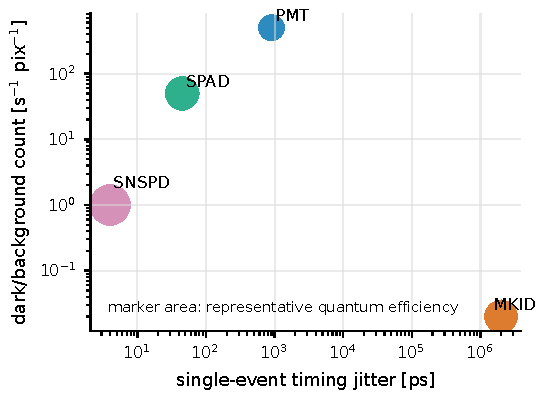
\includegraphics[width=0.70\linewidth]{figures/generated/chapter_06/ch06_detector_trade_space.pdf}
\caption{四类单光子探测技术的典型工作区域。横轴是单事件时间抖动，纵轴是每像素暗计数或背景计数的代表值，点面积表示代表性量子效率。PMT 适合大口径、高通量和 ns 级强度干涉；SPAD 给出几十皮秒计时但受面积和死时间限制；SNSPD 在低暗计数和皮秒计时上最强，但需要低温系统；MKID 牺牲时间分辨率，换取每个光子的能量信息和阵列化。}
\label{fig:ch06-detector-trade-space}
\end{figure}

效率决定事件数，死时间决定事件间隔统计是否还忠实于入射光场。非延长死时间模型给出
\begin{equation}
  R_{\rm obs}=\frac{R_{\rm in}}{1+R_{\rm in}\tau_d},
  \label{eq:ch06-nonparalyzable}
\end{equation}
\begin{formulaexplain}
\(R_{\rm in}\) 是入射事件率，\(R_{\rm obs}\) 是记录事件率，\(\tau_d\) 是死时间。非延长模型中，死时间内来的事件被丢弃，但不会延长探测器恢复时间。
\end{formulaexplain}
延长死时间模型给出
\begin{equation}
  R_{\rm obs}=R_{\rm in}\exp(-R_{\rm in}\tau_d).
  \label{eq:ch06-paralyzable}
\end{equation}
\begin{formulaexplain}
这也是死时间模型，但每个死时间内到来的新事件会重新触发恢复窗口。高通量时 \(R_{\rm obs}\) 可能先饱和再下降，因此必须知道真实探测器属于哪类响应。
\end{formulaexplain}
\(R_{\rm in}\) 和 \(R_{\rm obs}\) 的单位都是 s\(^{-1}\)，\(\tau_d\) 是死时间，单位秒。若 \(\tau_d=20\,{\rm ns}\)，非延长模型在 \(R_{\rm in}=10^7\,{\rm s^{-1}}\) 时已经让观测率比入射率低约 \(17\%\)；若 \(R_{\rm in}=10^8\,{\rm s^{-1}}\)，观测率接近饱和。SPAD 常见死时间为几十 ns 到几百 ns，MKID 可到 \(100\,\mu{\rm s}\) 量级，现代 TCSPC 电子学本身可以把通道死时间压到 650 ps，但探测器脉冲宽度和前端电子仍会限制真实高通量能力 \citep{2009A&A...508..531N,2013PASP..125.1348M,2020RScI...91a3108W}。

\begin{figure}[tbp]
\centering
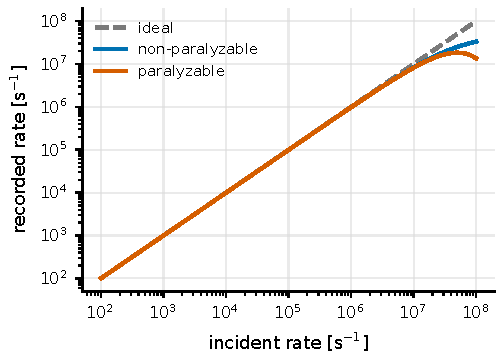
\includegraphics[width=0.70\linewidth]{figures/generated/chapter_06/ch06_deadtime_saturation.pdf}
\caption{入射计数率升高时，死时间使记录计数率偏离理想直线。非延长模型趋向饱和，延长模型在极高通量下反而下降。图中采用 \(\tau_d=20\,{\rm ns}\)，代表高速单光子通道的数量级；真实仪器需要用脉冲源或稳定光源单独测量 \(\tau_d\) 和模型类型。}
\label{fig:ch06-deadtime-saturation}
\end{figure}

afterpulsing 是另一种短延迟污染。雪崩器件中滞留载流子会在主脉冲后释放，产生与真实天体光子无关的二次事件。若每个真实事件产生 afterpulse 的概率为 \(\epsilon_{\rm ap}\)，延迟分布为归一化核 \(k_{\rm ap}(\tau)\)，额外事件率可写成
\begin{equation}
  R_{\rm ap}(\tau)=\epsilon_{\rm ap}\,R_{\rm det}\,k_{\rm ap}(\tau),
  \qquad
  \int_0^\infty k_{\rm ap}(\tau)\,d\tau=1.
  \label{eq:ch06-afterpulse}
\end{equation}
\begin{formulaexplain}
\(R_{\rm ap}\) 是 afterpulse 贡献；\(\epsilon_{\rm ap}\) 是每个真实事件产生伪脉冲的概率；\(k_{\rm ap}\) 是归一化延迟核。它描述探测器自身制造的短延迟假相关。
\end{formulaexplain}
\(\epsilon_{\rm ap}\) 无量纲，常在 \(10^{-4}\)--\(10^{-2}\) 范围内随器件和门控方式变化；\(k_{\rm ap}\) 的特征时间可从 ns 到 \(\mu{\rm s}\)。同一探测器的自相关会直接看到 afterpulse 峰，两个独立探测器的互相关则大幅降低这类污染。HBT 分束和多通道交叉相关因此有两层作用：提高可承受计数率，同时压制同通道死时间和 afterpulsing \citep{1957RSPSA.242..300B,1996ApOpt..35.1956C,2020RScI...91a3108W}。

\Needspace{14\baselineskip}
时间响应把真实相关峰卷积成更宽的峰。若两个通道的时间响应分别为 \(h_1(t)\) 和 \(h_2(t)\)，观测到的二阶相关超额近似为
\begin{equation}
  C^{\rm obs}_{12}(\tau)
  =
  \int C^{\rm sky}_{12}(\tau')\,
  h_{12}(\tau-\tau')\,d\tau',
  \qquad
  h_{12}=h_1*h_2.
  \label{eq:ch06-response-convolution}
\end{equation}
\begin{formulaexplain}
\(C^{\rm sky}_{12}\) 是天体真实相关，\(C^{\rm obs}_{12}\) 是观测结果；\(h_1,h_2\) 是两通道时间响应，\(h_{12}\) 是合成响应。仪器会把窄相关峰卷积展宽。
\end{formulaexplain}
\(C_{12}=g^{(2)}_{12}-1\) 无量纲，\(\tau\) 和 \(\tau'\) 的单位是秒。若响应函数近似高斯，宽度预算可写成
\begin{equation}
  \sigma_{\rm obs}^2
  \simeq
  \sigma_{\rm sky}^2+\sigma_1^2+\sigma_2^2+\sigma_{\rm opt}^2+\sigma_{\rm clk}^2 .
  \label{eq:ch06-jitter-budget}
\end{equation}
\begin{formulaexplain}
\(\sigma_{\rm obs}\) 是观测峰宽；\(\sigma_{\rm sky}\) 是源自身宽度；\(\sigma_1,\sigma_2\)、\(\sigma_{\rm opt}\)、\(\sigma_{\rm clk}\) 分别来自探测器、光路和时钟。独立高斯展宽按方差相加。
\end{formulaexplain}
\(\sigma_{\rm sky}\) 是光源自身相干时间或脉冲宽度，\(\sigma_1,\sigma_2\) 是探测器和电子通道的 rms 抖动，\(\sigma_{\rm opt}\) 是镜面等时性和光路展宽，\(\sigma_{\rm clk}\) 是两站时钟残差。VERITAS 的 Davies-Cotton 镜面和 PMT 脉冲宽度使强度相关峰可用 \(\sigma_\tau\simeq4\,{\rm ns}\) 的高斯描述；MAGIC-SII 相关峰的高斯宽度约 \(2.2\,{\rm ns}\)，并用自相关长期跟踪电子带宽稳定性 \citep{2020NatAs...4.1164A,2024MNRAS.529.4387A}。

\begin{figure}[tbp]
\centering
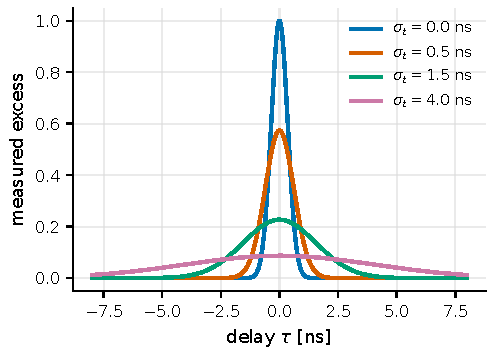
\includegraphics[width=0.70\linewidth]{figures/generated/chapter_06/ch06_detector_timing_response.pdf}
\caption{有限时间响应会把窄相关峰展宽并降低峰高。曲线保持峰面积近似不变，只改变 rms 抖动 \(\sigma_t\)。当真实相干时间远短于 ns 级电子响应时，峰宽主要由仪器决定，峰高按展宽因子被稀释；这正是强度干涉中需要高电子带宽和稳定响应函数的原因。}
\label{fig:ch06-detector-timing-response}
\end{figure}

\section{时钟和几何延迟怎样建立共同时间轴}

两台望远镜的事件表只有放到共同时间轴上才可以相关。短基线强度干涉主要要求相对延迟稳定，脉冲星计时、快速暂现源和跨夜合并还要求绝对时间可追溯到标准时间尺度。AquEYE/Iqueye 采用铷钟和 GPS PPS，把相对时间精度做到约 100 ps rms，把绝对 UTC 精度控制在 \(0.5\,{\rm ns}\) 以内；现代多通道时间标记器可接入 White Rabbit 光纤网络，5 km 光纤链路测试得到约 39 ps 的同步贡献 \citep{2009A&A...508..531N,2015SPIE.9504E..0CZ,2013NIMPA.725..187J,2020RScI...91a3108W}。

\Needspace{13\baselineskip}
对一对站点 \(a,b\)，几何延迟为
\begin{equation}
  \Delta t_{\rm geo}(t)
  =
  \frac{\mathbf{B}_{ab}(t)\cdot\hat{\mathbf{s}}}{c},
  \qquad
  \mathbf{B}_{ab}=\mathbf{r}_b-\mathbf{r}_a .
  \label{eq:ch06-geometric-delay}
\end{equation}
\begin{formulaexplain}
\(\Delta t_{\rm geo}\) 是两站几何延迟；\(\mathbf B_{ab}\) 是基线向量，\(\hat{\mathbf s}\) 是源方向，\(c\) 是光速。它把空间基线投影成两路事件表需要相互平移的时间量。
\end{formulaexplain}
\(\mathbf{B}_{ab}\) 的单位是 m，\(\hat{\mathbf{s}}\) 无量纲，\(\Delta t_{\rm geo}\) 的单位是秒。地球自转会让投影基线随时间变化，所以几何延迟也随时间漂移。一个 100 m 基线在天顶附近的延迟变化速度约为 \(\Omega_\oplus B/c\sim2.4\times10^{-11}\,{\rm s\,s^{-1}}\)，17 分钟内可漂移几十 ps；对 km 基线或皮秒级相关峰，这个变化不能只用一个常数延迟吸收。VERITAS-SII 对每个相关帧移动时间 lag 来校正几何光程，MAGIC-SII 在 Pearson 相关后应用可变时间延迟校正 \citep{2020NatAs...4.1164A,2024MNRAS.529.4387A}。

若要把事件折叠到脉冲星相位，或把光子到达时刻与其他波段比较，站点时间还要转换到太阳系质心。概念上可写为
\begin{equation}
  t_{\rm SSB}
  =
  t_{\rm site}
  +\Delta_{\rm C}
  +\Delta_{\rm R}
  +\Delta_{\rm E}
  +\Delta_{\rm S}
  +\Delta_{\rm A}.
  \label{eq:ch06-barycentric-time}
\end{equation}
\begin{formulaexplain}
\(t_{\rm SSB}\) 是太阳系质心到达时；\(t_{\rm site}\) 是站点时间；各 \(\Delta\) 项修正时钟、Roemer、Einstein、Shapiro 和大气延迟。它用于跨夜、跨波段和脉冲相位比较。
\end{formulaexplain}
\(\Delta_{\rm C}\) 是本地时钟到标准原子时和坐标时的校正，包含 UTC 到 TAI、TT、TDB 或 TCB 的时间尺度转换和闰秒；\(\Delta_{\rm R}\) 是 Roemer 光行时，地球绕太阳运动给出最高约 \(\pm500\,{\rm s}\) 的投影项；\(\Delta_{\rm E}\) 是 Einstein 延迟，来自引力势和运动导致的钟速变化；\(\Delta_{\rm S}\) 是太阳系天体的 Shapiro 延迟；\(\Delta_{\rm A}\) 是大气传播延迟。Tempo2 把这些项实现到 ns 级，barycorrpy 和 Astropy 则给出 Python 工作流中的时间尺度和质心速度/时间改正接口 \citep{2006MNRAS.369..655H,2006MNRAS.372.1549E,2018RNAAS...2....4K,2013A&A...558A..33A,2018AJ....156..123A}。

\begin{figure}[tbp]
\centering
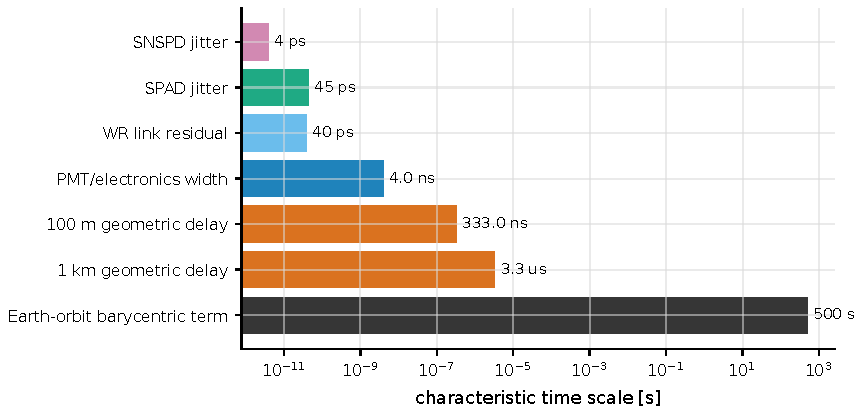
\includegraphics[width=0.82\linewidth]{figures/generated/chapter_06/ch06_time_budget.pdf}
\caption{同一份事件表会同时遇到皮秒、纳秒、微秒和百秒量级的时间项。探测器抖动和 White Rabbit 残差决定相关峰能否保持窄形；电子和镜面响应决定 ns 级强度干涉峰宽；几何延迟由基线长度和源方向决定；太阳系质心改正虽然对同夜强度相关不是峰宽项，却是脉冲星相位、跨夜合并和多信使比较的绝对时间基础。}
\label{fig:ch06-time-budget}
\end{figure}

\Needspace{16\baselineskip}
\section{光谱、偏振和背景为什么也要进事件表}

窄带滤光片、分色镜、光纤光谱仪和 MKID 都是在事件表里给每个光子增加频率信息。光谱通道的中心波长 \(\lambda\)、宽度 \(\Delta\lambda\) 和形状 \(S(\lambda)\) 决定相干时间。若通道近似矩形，数量级关系为
\begin{equation}
  \tau_c
  \simeq
  \frac{1}{\Delta\nu}
  \simeq
  \frac{\lambda^2}{c\,\Delta\lambda}
  =
  \frac{R\,\lambda}{c},
  \qquad
  R=\frac{\lambda}{\Delta\lambda}.
  \label{eq:ch06-coherence-time}
\end{equation}
\begin{formulaexplain}
\(\tau_c\) 是相干时间；\(\Delta\nu\) 是频率带宽；\(\lambda,\Delta\lambda\) 是中心波长和带宽；\(R\) 是光谱分辨率。窄通道让相位记忆变长，但单通道光子率变低。
\end{formulaexplain}
\(\tau_c\) 的单位是秒。以 \(\lambda=500\,{\rm nm}\) 为例，\(R=100\) 给出 \(\tau_c\simeq0.17\,{\rm ps}\)，\(R=10^4\) 给出 \(\tau_c\simeq17\,{\rm ps}\)，\(R=10^5\) 给出 \(\tau_c\simeq170\,{\rm ps}\)。这些数仍短于多数 PMT/电子链的 ns 响应，所以实际相关峰宽通常由仪器决定，峰高则包含电子带宽与光学带宽的比值。VERITAS 使用中心 416 nm、有效宽度 13 nm 的滤光片；MAGIC 使用 425 nm、26 nm 干涉滤光片，但快光束入射角会改变实际通带形状 \citep{2020NatAs...4.1164A,2024MNRAS.529.4387A,1974iiia.book.....H}。

\begin{figure}[tbp]
\centering
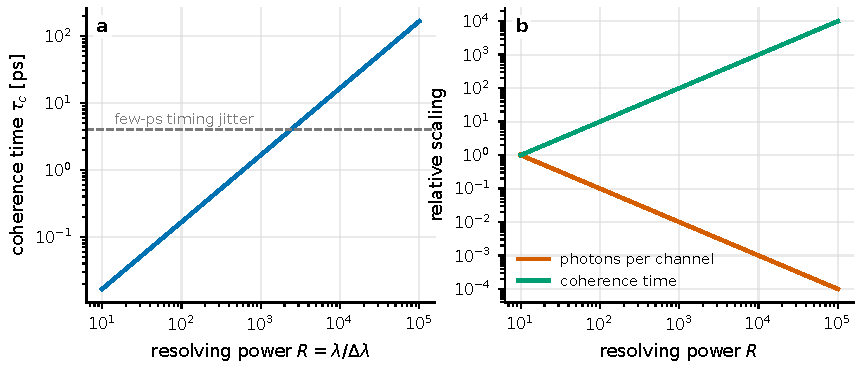
\includegraphics[width=0.92\linewidth]{figures/generated/chapter_06/ch06_spectral_resolution_coherence.pdf}
\caption{光谱分辨率和相干时间的数量级关系。左图固定 \(\lambda=500\,{\rm nm}\)，显示 \(\tau_c\simeq R\lambda/c\) 随分辨率线性增长；右图显示单个通道的光子率约随 \(1/R\) 降低，而相干时间随 \(R\) 增加。理想强度干涉信噪比对光学带宽的依赖会部分抵消，但真实仪器还受到滤光片形状、探测器响应、背景和电子带宽限制。}
\label{fig:ch06-spectral-resolution-coherence}
\end{figure}

提高 \(R\) 会拉长 \(\tau_c\)，但会减少单通道光子率；若要保留总通量，需要同时读出更多波长通道。多通道 TCSPC 可以把不同波长通道作为独立输入，并输出单一时间排序的数据流；MAGIC 和 VERITAS 的 SII 系统则选择少数宽滤光片通道换取更高光子率 \citep{2020RScI...91a3108W,2020NatAs...4.1164A,2024MNRAS.529.4387A}。对恒星直径测量，宽通道提高信噪比；对发射线、吸收线、快速旋转星或风结构，分波长相关可能直接给出空间信息随速度的变化。

偏振通道记录的是电场方向的投影。若仪器把两个正交线偏振 \(H,V\) 分开，最简单的计数估计为
\begin{equation}
  I=R_H+R_V,\qquad Q=R_H-R_V .
  \label{eq:ch06-stokes-hv}
\end{equation}
\begin{formulaexplain}
\(R_H,R_V\) 是两个正交线偏振通道的计数率；\(I\) 是总强度，\(Q\) 是水平和垂直偏振差。分偏振事件表可以在后处理中重建 Stokes 信息。
\end{formulaexplain}
若再用 \(45^\circ/135^\circ\) 和左/右圆偏振通道，可估计 \(U\) 和 \(V\)。这里的 \(R_p\) 是偏振通道 \(p\) 的背景扣除计数率，单位 s\(^{-1}\)。真实仪器还要引入 Mueller 矩阵 \(M_{ij}\)，把望远镜反射、偏振片消光比、波片相位误差和探测器效率差写成
\begin{equation}
  \mathbf{S}_{\rm obs}=M\,\mathbf{S}_{\rm sky}+\mathbf{b},
  \label{eq:ch06-mueller}
\end{equation}
\begin{formulaexplain}
\(\mathbf S_{\rm sky}\) 和 \(\mathbf S_{\rm obs}\) 是天空与观测 Stokes 向量；\(M\) 是仪器 Mueller 矩阵；\(\mathbf b\) 是背景偏置。它把偏振串扰和效率差写成可标定模型。
\end{formulaexplain}
\(\mathbf{S}=(I,Q,U,V)^T\)，\(\mathbf{b}\) 是背景和偏置。偏振强度干涉可以比较 \(HH\) 或 \(VV\) 的相关，也可以构造交叉偏振相关，用来区分天体偏振结构和仪器串扰；一旦事件表只保存总光强，这些检验就无法重新执行。

通量和背景也必须随时间进入元数据。式 \eqref{eq:ch06-detected-rate} 中的 \(R_{\rm sky}\) 会随月相、云、视场、滤光片和地平高度变化。对大气 Cherenkov 望远镜，亮月期间反而常常是 SII 的可用时间，因为 gamma-ray 模式受夜天光限制会停观；但夜天光进入 PMT 后仍会稀释恒星相关。若 \(\beta_i=R_{{\rm bkg},i}/R_{*,i}\)，两台望远镜的背景稀释因子近似为
\begin{equation}
  |g^{(1)}_*|^2
  \simeq
  |g^{(1)}_{\rm meas}|^2
  (1+\beta_1)(1+\beta_2),
  \label{eq:ch06-background-dilution}
\end{equation}
\begin{formulaexplain}
\(|g_*^{(1)}|^2\) 是扣除背景后的恒星平方相干度；\(|g_{\rm meas}^{(1)}|^2\) 是测得值；\(\beta_i\) 是第 \(i\) 台望远镜的背景/恒星计数比。背景会把真实相关稀释掉。
\end{formulaexplain}
前提是恒星-背景和背景-背景起伏在两站之间不相关。这个式子里的 \(R_*\) 和 \(R_{\rm bkg}\) 应来自同一通道、同一增益状态和相近时间的测量；否则背景修正会把慢变增益误认为天体相关幅度 \citep{2020NatAs...4.1164A,2024MNRAS.529.4387A}。

\section{标定和数据格式怎样保证可复现}

探测器响应要先在实验室和天空上固定下来。暗场给出 \(R_{\rm dark}\) 和热背景；稳定连续光源给出线性范围和死时间曲线；弱脉冲激光给出 \(h(t)\)、通道间固定延迟和时间 walk；分束到两个独立探测器的零基线实验给出电子相关峰和 afterpulsing 的区别。对强度干涉，错延迟、错偏振、off-source 背景和远离零延迟的 lag 都应作为 null test。VERITAS-SII 在每个 1 s 相关帧中剔除高频电子噪声污染，MAGIC-SII 用无光子输入和远离信号延迟的相关来估计残余电子相关，并用自相关监测电子带宽稳定性 \citep{2020NatAs...4.1164A,2024MNRAS.529.4387A}。

时间和坐标元数据决定这些标定几年后还能不能复现。一个可复现的事件表至少应保存：站点地理坐标和高度；望远镜姿态和基线；原始时钟源、频率标准、闰秒表版本和时间尺度；每个通道的电子延迟、探测器偏置、高压、温度和死时间模型；滤光片或光谱响应曲线；偏振模块角度和 Mueller 标定；质量标记定义；软件版本和选择条件。FITS 标准允许用 BINTABLE 扩展保存 time-tagged photon events，并用 header 关键字描述数据含义；Astropy 提供 FITS、坐标和时间处理接口，适合把事件表、时间尺度转换和质心改正放入同一 Python 分析链 \citep{2010A&A...524A..42P,2013A&A...558A..33A,2018AJ....156..123A}。

FITS 适合长期归档和与天文软件互操作，HDF5 或 Parquet 适合高吞吐量分析和列式筛选。无论格式如何，原始事件、标定事件和相关产品最好分层保存。原始层不可被后处理覆盖；标定层记录每个版本的校正结果；相关产品层记录 bin 宽、延迟网格、权重、剔除条件和协方差。这样，一个读者可以从同一份原始数据重新生成光变曲线、\(g^{(2)}(\tau)\)、空间可见度或脉冲到达时刻，而不需要猜测早期分析脚本做了哪些隐含选择。

